\let\negmedspace\undefined
\let\negthickspace\undefined
\documentclass[journal]{IEEEtran}
\usepackage[a5paper, margin=10mm, onecolumn]{geometry}
%\usepackage{lmodern} % Ensure lmodern is loaded for pdflatex
\usepackage{tfrupee} % Include tfrupee package

\setlength{\headheight}{1cm} % Set the height of the header box
\setlength{\headsep}{0mm}     % Set the distance between the header box and the top of the text

\usepackage{gvv-book}
\usepackage{gvv}
\usepackage{cite}
\usepackage{amsmath,amssymb,amsfonts,amsthm}
\usepackage{algorithmic}
\usepackage{graphicx}
\usepackage{textcomp}
\usepackage{xcolor}
\usepackage{txfonts}
\usepackage{listings}
\usepackage{enumitem}
\usepackage{mathtools}
\usepackage{gensymb}
\usepackage{comment}
\usepackage[breaklinks=true]{hyperref}
\usepackage{tkz-euclide} 
\usepackage{listings}
% \usepackage{gvv}                                        
\def\inputGnumericTable{}                                 
\usepackage[latin1]{inputenc}                                
\usepackage{color}                                            
\usepackage{array}                                            
\usepackage{longtable}                                       
\usepackage{calc}                                             
\usepackage{multirow}                                         
\usepackage{hhline}                                           
\usepackage{ifthen}                                           
\usepackage{lscape}
\begin{document}

\bibliographystyle{IEEEtran}
\vspace{3cm}

\title{NCERT-12.8.ex.14}
\author{EE24BTECH11043 - Murra Rajesh Kumar Reddy}

% \maketitle
% \newpage
% \bigskip
{\let\newpage\relax\maketitle}

\renewcommand{\thefigure}{\theenumi}
\renewcommand{\thetable}{\theenumi}
\setlength{\intextsep}{10pt} % Space between text and floats


\numberwithin{equation}{enumi}
\numberwithin{figure}{enumi}
\renewcommand{\thetable}{\theenumi}
\textbf{Question:} \\
Find the area of the given region : \\
$\cbrak{\brak{x,y}:0 \le y \le x^2+1, 0 \le y \le x+1, 0 \le x \le 2 }$ \\
\textbf{Solution}: \\
\textbf{Theoretical Solution}: \\
Given regions are,
\begin{align}
A_1 = \cbrak{\brak{x,y}:0 \le y \le x^2+1} \\
A_2 = \cbrak{\brak{x,y}: 0 \le y \le x+1} \\
A_3 = \cbrak{\brak{x,y}: 0 \le x \le 2}
\end{align}
Let's say the area we need to find is of function $f\brak{x}$ within the limits of $a$ and $b$ along $x$-axis then the required area is given by
\begin{align}
	Area = \int_{a}^{b} f\brak{x} dx
\end{align}
From the equation $\brak{0.3}$ we can say 
\begin{align}
	a = 0 \\
	b = 2
\end{align}
From equations  $\brak{0.1}$ and $\brak{0.2}$ we can say point of intersection of $A_1$ and $A_2$ is
\textbf{Point of intersection}\\
Expressing the equation of parabola in matrix form $g\brak{\vec{x}}= \vec{x}^{\top}\vec{V}\vec{x}+2\vec{u}^{\top}\vec{x}+f=0$,
\begin{align}
  \myvec{x&y}\myvec{1&0\\0&0}\myvec{x\\y}+2\myvec{0 & -\frac{1}{2}}\myvec{x\\y}+1=0
\end{align}
The general form of a line equation can be expressed as
\begin{align}
    \vec{m}^\top \vec{x} = c
\end{align}
For $y=x+1$
\begin{align}
    \vec{m} = \begin{pmatrix} -1 \\ 1 \end{pmatrix}, \quad c = 1
\end{align}
Intersection of a line and a conic is given by,
\begin{align}
  \kappa_i=\frac{-\vec{m}^{\top}\brak{\vec{Vh}+\vec{u}}\pm\sqrt{\sbrak{\vec{m}^{\top}\brak{\vec{Vh}+\vec{u}}}^2-g\brak{h}\brak{\vec{m}^{\top}\vec{Vm}}}}{\vec{m}^{\top}\vec{Vm}}
\end{align}
On substituting and solving \\
The intersection point is $\brak{1,2}$ and
$f\brak{x}$ will be
\begin{align}
	f\brak{x} = x^2 +1  && \brak{0 \le x \le 1} \\
	f\brak{x} = x+1 && \brak{1 \le x \le 2} \\
	Area = \int_{0}^{1}\brak{x^2+1} dx + \int_{1}^{2} \brak{x+1} dx
\end{align}
By computing each integral we get
\begin{align}
	\int_{0}^{1}\brak{x^2+1} dx = \sbrak{\frac{x^3}{3} + x}_{0}^{1} = \sbrak{\frac{4}{3} -0 } = \frac{4}{3} \\
	\int_{1}^{2}\brak{x+1} dx = \sbrak{\frac{x^2}{2} + x}_{1}^{2} = \sbrak{4 - \frac{3}{2}} = \frac{5}{2}
\end{align}
From the equations \brak{0.10} and \brak{0.11} 
\begin{align}
	Area = \frac{23}{6} = 3.83
\end{align}
Total area of given regions is $\frac{23}{6}$ \\
\textbf{Computational Solution}: \\
\textbf{Logic}: \\
According trapezoidal rule the given integral will be:
\begin{align}
	\int_{a}^{b} f\brak{x} dx \approx \sigma_{k = 1}^{N} \frac{f\brak{x_{k+1} + f\brak{x_k}}}{2} h && h = \frac{b-a}{N}
\end{align}
$\therefore$ The equation obtained is
\begin{align}
	Area = \int_{a}^{b} f\brak{x} dx \approx h\brak{\frac{1}{2}f\brak{a}+f\brak{x_1}+ f\brak{x_2} + \dots + f\brak{x_n-1}+\frac{1}{2}f\brak{b}} \\
	Area = j_n \quad \brak{j_{i+1} = j_i + h\frac{f\brak{x_{i+1} + f\brak{x_i}}}{2}} \\
	Area = j_n \quad \brak{j_{i+1} = j_i +h\frac{\brak{x_{i+1}^2+1} +\brak{x_i^2 +1}}{2}} && 0 \le x \le 1 \\
	Area = j_n \quad \brak{j{i+1} = j_i + h\frac{\brak{x_{i+1}+1}+\brak{x_i}+1}{2}} && 1 \le x \le 2 \\
	x_{i+1} = x_{i} + h \\
	N = 100000
\end{align}
Using the code the answer we get is
\begin{figure}[H]
	\centering
	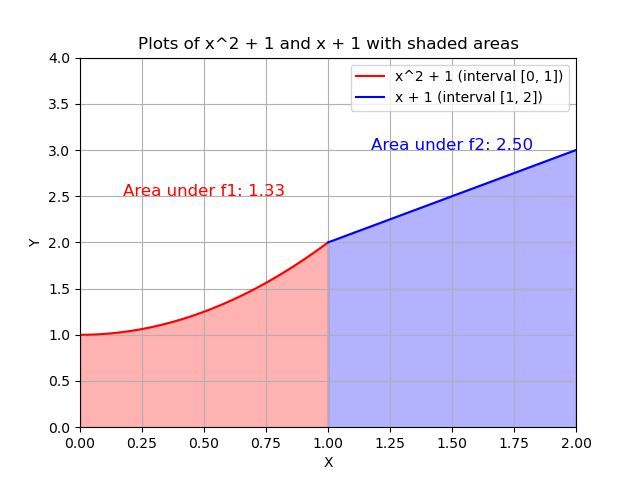
\includegraphics[width = \columnwidth]{figs/Figure_1.png}
	\label{fig}
\end{figure}
Area calculated by computaional method = Area under $f_1$ + Area under $f_2$ \\
\begin{align}
Area = 1.33 + 2.5 = 3.83
\end{align}
We got same answer from Theoretical solution also . So we can say our computation is correct.
\end{document}

